\documentclass[report.tex]{subfiles}
\begin{document}
\section{Baseline without Middleware (75 pts)}\label{exp2}

In this section the performance characteristics of the memtier clients and memcached servers in the azure cloud are studied.

\subsection{One Server}\label{exp21}

%Both, for a read-only and write-only workload plot the throughput and the response time as a function of NumClients. All clients are connected to a single memcached instance.

%Use 3 load generating VMs, with one memtier (CT=2) each, and vary the number of virtual clients (VC) per memtier thread between 1 and 32. Show how the behavior of the server changes as we add more clients.

This experiment analyses the behaviour of the system with 3 load generating VM's and a single server VM. The detailed experiment configuration is presented in the table below.

For every configuration the throughput and response time as measured on the client is used.

Every graph contains the sample standard deviation over the 3 repetitions as an error metric.
To validate the measurements the interactive law with a client thinking time Z of 0 is shown in every throughput and response time graph.

As mentioned in section \ref{simulation} before running the experiment the network bandwidth between the VM's was tested using \emph{iperf}. From these measurements a maximal achievable throughput was derived by considering the value size of 4096B. This bandwidth limit is also shown in the throughput graphs.


\begin{center}
	\scriptsize{
		\begin{tabular}{|l|c|}
			\hline Number of servers                & 1                        \\ 
			\hline Number of client machines        & 3                        \\ 
			\hline Instances of memtier per machine & 1                        \\ 
			\hline Threads per memtier instance     & 2                        \\
			\hline Virtual clients per thread       & [1, 2, 4, 8, 12, 16, 24, 32]\\ 
			\hline Workload                         & Write-only and Read-only \\
			%\hline Multi-Get behavior               & N/A                      \\
			%\hline Multi-Get size                   & N/A                      \\
			%\hline Number of middlewares            & N/A                      \\
			%\hline Worker threads per middleware    & N/A                      \\
			\hline Repetitions                      & 3 (at least 1 minute each)\\ 
			\hline 
		\end{tabular}
	}
\end{center}


\begin{figure}
	\begin{subfigure}[b]{.49\linewidth}
		\centering
		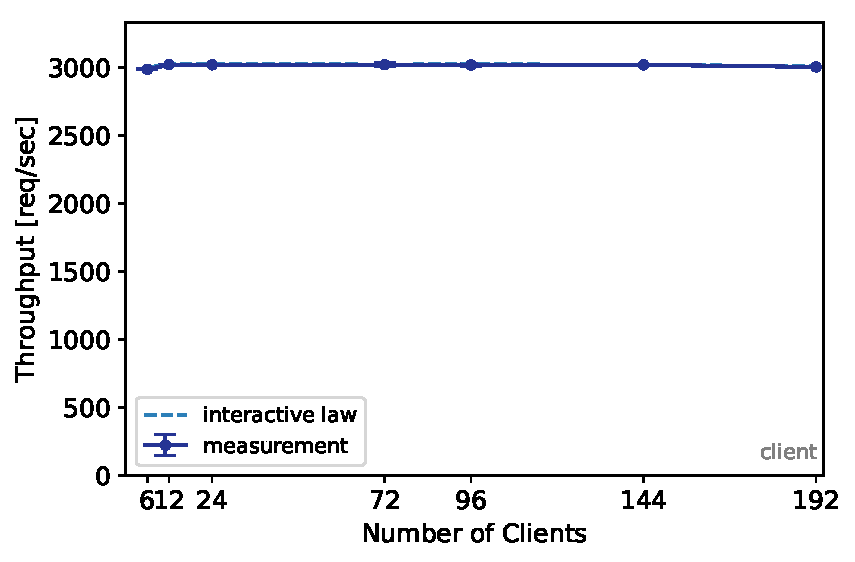
\includegraphics[width=\linewidth]{data/exp21_ro_tp_nc.pdf}
	\end{subfigure}\hfill
	\begin{subfigure}[b]{.49\linewidth}
		\centering
		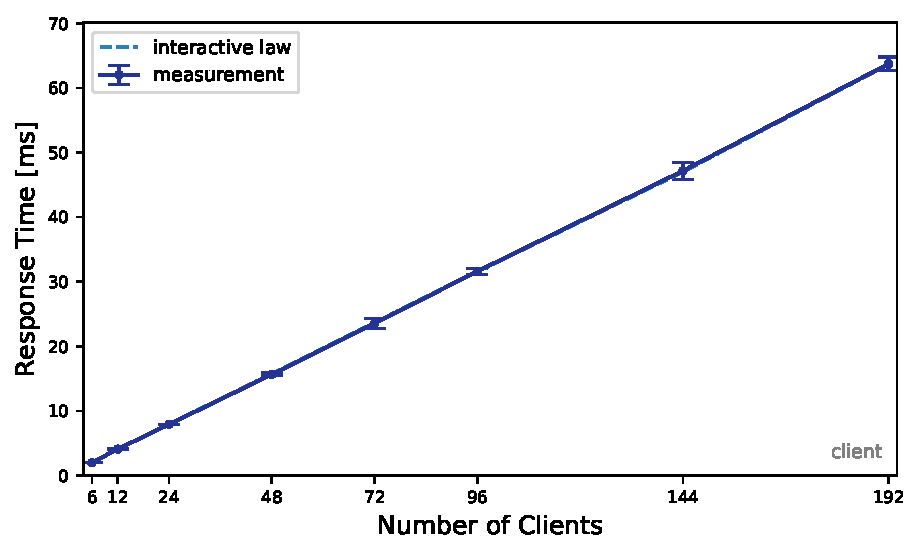
\includegraphics[width=\linewidth]{data/exp21_ro_rt_nc.pdf}
	\end{subfigure}%
	\caption{Throughput and response time with interactive law in read-only workload with one memcached server.}
	\label{exp21_ro_nc}
\end{figure}


\begin{figure}
	\begin{subfigure}[b]{.49\linewidth}
		\centering
		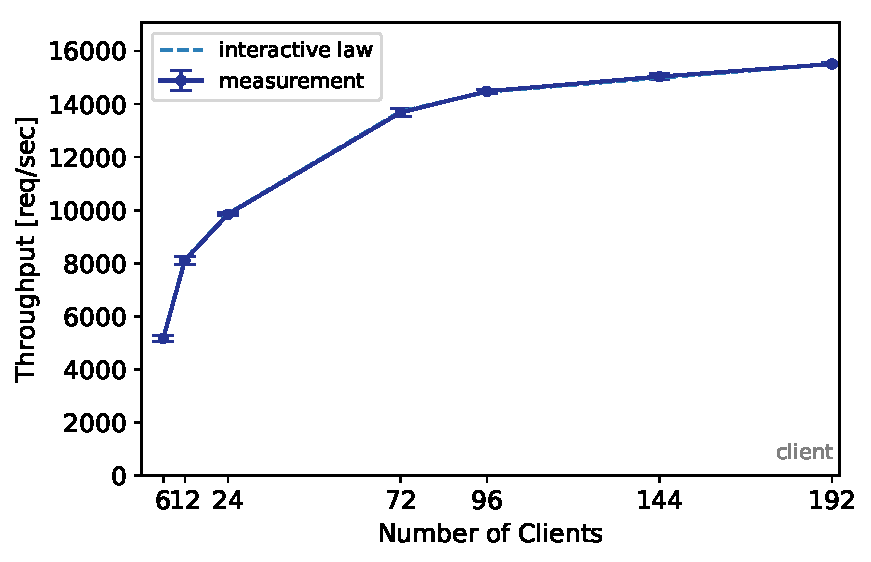
\includegraphics[width=\linewidth]{data/exp21_wo_tp_nc.pdf}
	\end{subfigure}\hfill
	\begin{subfigure}[b]{.49\linewidth}
		\centering
		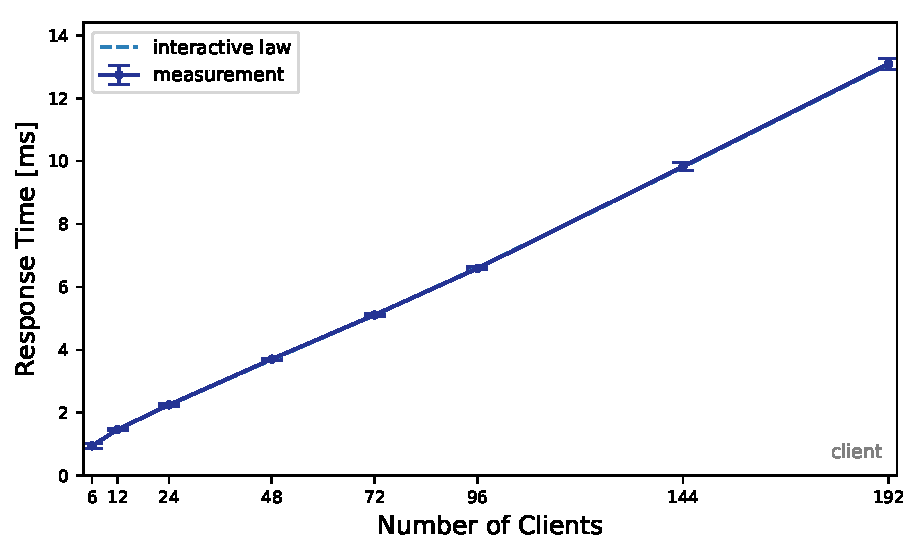
\includegraphics[width=\linewidth]{data/exp21_wo_rt_nc.pdf}
	\end{subfigure}%
	\caption{Throughput and response time with interactive law in write-only workload with one memcached server.}
	\label{exp21_wo_nc}
\end{figure}



\subsubsection{Explanation}

%Describe in which phase the memcached servers are under-saturated, saturated, or over-saturated. Describe how throughput and response time correlate. Explain what further conclusions can be drawn from the experiment.

As shown in figure \ref{exp21_ro_nc}, the throughput saturation for the read-only workload is already reached at 6 clients because the upload bandwidth of the single server VM limits the throughput. Before the experiment, the server VM upload bandwidth was measured to be 99.6 MBit/sec. When using a value size of 4096B, this results in a maximum possible throughput of 3040 ops/sec for a read-only workload because all the values need to be sent from the server VM to one of the 3 client VM's. 

Consequently increasing the number of clients has almost no effect on the throughput while the response time grows linearly because more clients results in more requests on the server that wait to be sent to a client VM. \todo{maybe be more precice about why linear increase: I think more clients => more requests => every request needs to "wait" a bit longer on server vm}

In figure \ref{exp21_wo_nc} it can be observed that for a write-only workload the throughput saturation is reached at 72 clients. In this experiment the bottleneck is not the bandwidth but rather the memcached server. 
As expected the throughput first increases in the number of clients while the memcached servers are still under-saturated and then the response 


\subsection{Two Servers}\label{exp22}

%For a read-only and write-only workload plot throughput and response time as a function of NumClients. The clients are connected to two memcached instances. 

%Use 1 load generating VM, with one memtier (CT=1) connected to each memcached instance (two memcache instances in total), and vary the number of virtual clients (VC) per memtier thread between 1 and 32. Show how the behavior of the server changes and explain what conclusions we can draw from this experiment.

\begin{center}
	\scriptsize{
		\begin{tabular}{|l|c|}
			\hline Number of servers                & 2                        \\ 
			\hline Number of client machines        & 1                        \\ 
			\hline Instances of memtier per machine & 2                        \\ 
			\hline Threads per memtier instance     & 1                        \\
			\hline Virtual clients per thread       & [1, 2, 4, 8, 12, 16, 24, 32]\\ 
			\hline Workload                         & Write-only and Read-only \\
			%\hline Multi-Get behavior               & N/A                      \\
			%\hline Multi-Get size                   & N/A                      \\
			%\hline Number of middlewares            & N/A                      \\
			%\hline Worker threads per middleware    & N/A                      \\
			\hline Repetitions                      & 3 (at least 1 minute each) \\ 
			\hline 
		\end{tabular}
	} 
\end{center}



\begin{figure}
	\begin{subfigure}[b]{.49\linewidth}
		\centering
		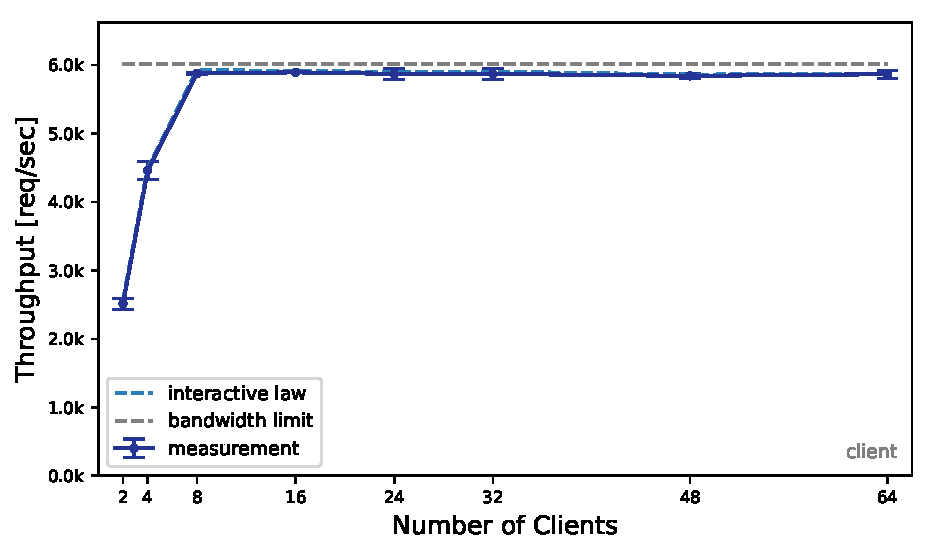
\includegraphics[width=\linewidth]{data/exp22_ro_tp_nc.pdf}
	\end{subfigure}\hfill
	\begin{subfigure}[b]{.49\linewidth}
		\centering
		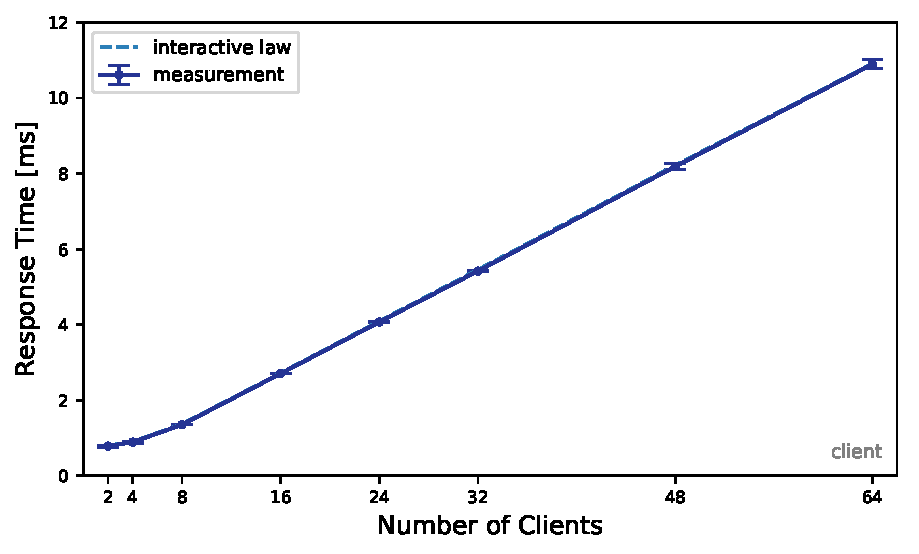
\includegraphics[width=\linewidth]{data/exp22_ro_rt_nc.pdf}
	\end{subfigure}%
	\caption{Throughput and response time with interactive law in read-only workload with one load generating VM.}
	\label{exp22_ro_nc}
\end{figure}




\begin{figure}
	\begin{subfigure}[b]{.49\linewidth}
		\centering
		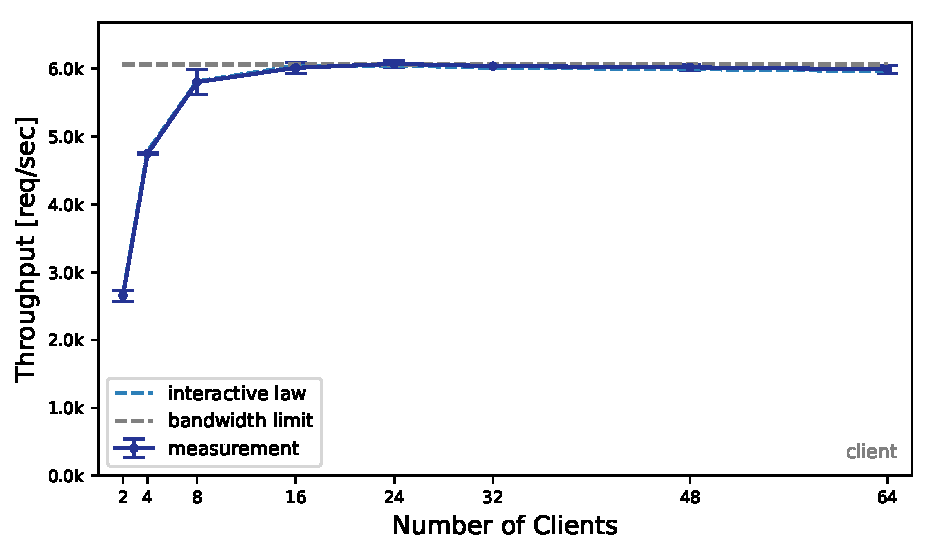
\includegraphics[width=\linewidth]{data/exp22_wo_tp_nc.pdf}
	\end{subfigure}\hfill
	\begin{subfigure}[b]{.49\linewidth}
		\centering
		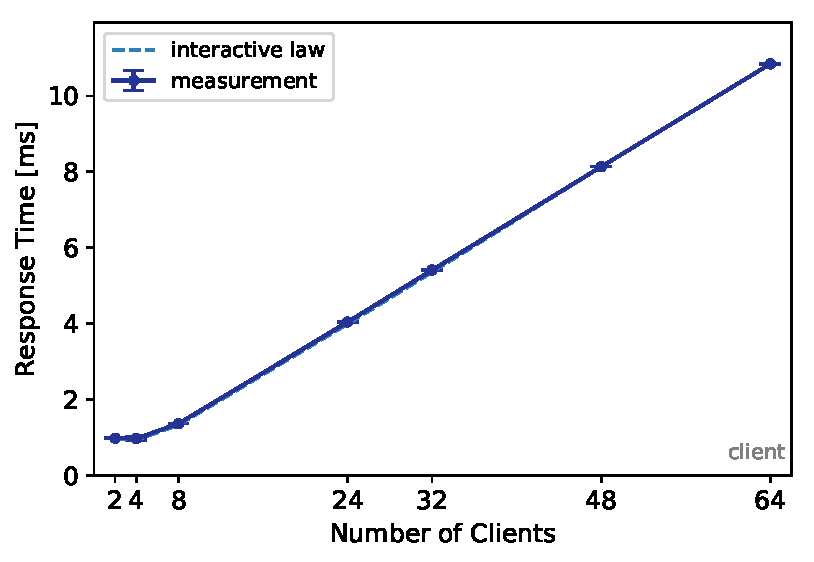
\includegraphics[width=\linewidth]{data/exp22_wo_rt_nc.pdf}
	\end{subfigure}%
	\caption{Throughput and response time with interactive law in write-only workload with one load generating VM.}
	\label{exp22_wo_nc}
\end{figure}



\subsubsection{Explanation}

%Describe how this experiment compares to the previous section. Which results are the same and which ones differ? Explain what further conclusions can be drawn from the experiment.

For a read-only workload the throughput saturation is reached at 8 clients, as shown in figure \ref{exp22_ro_nc}, because the upload bandwidth of the two servers limits the possible throughput. The measured total upload bandwidth between the 2 server VM's and the client VM is 199 MBit/sec which results in an estimate of 6062 ops/sec for the maximally achievable throughput when using values of 4096B. Before the saturation point is reached at 8 clients, increasing the number of clients results in a higher throughput as expected because the system is still under-saturated. \todo{maybe mention that because cutoff is so abruptly that it could be expected that with 8 clients memcached itself is not saturated at all}

Using a write-only workload with values of 4096B the situation is similar but here instead of the upload bandwidth of the server VM's the bottleneck is the upload bandwidth of the load generating client VM. The measured 199 MBit/sec total upload bandwidth of the client VM limits the throughput of the system to 6062 ops/sec. So as a consequence  the throughput saturation is reached at \todo{choose either 8 or 16} clients as shown in figure \ref{exp22_wo_nc}.


\subsection{Summary}


\begin{center}
	{Maximum throughput of different VMs.}
	\begin{tabular}{|l|p{2cm}|p{2cm}|p{4cm}|}
		\hline                        & Read-only workload & Write-only workload & Configuration gives max. throughput \\ 
		\hline One memcached server   & 2962 ops/sec       & 14097 ops/sec & 6 clients for read-only 72 clients for write-only\\ 
		\hline One load generating VM & 5878 ops/sec       &  5802 or 6012 ops/sec & 8 clients for read-only 8/16 clients for write-only\\ 
		\hline 
	\end{tabular}
\end{center}


%Write at least two paragraphs about how both results relate. Describe what is the bottleneck of this setup is. If the maximum throughput for both experiments is the same, explain why. If it is not the case, explain why not. Write down key take-away messages about the behaviour of the memtier clients and the memcached servers.

\paragraph{Comparison of one memcached server vs. one load generating VM}
For a read-only workload both experiments are bound by the network upload bandwidth of the server VM(s).
Despite the fact that they are both network bound, they have a different maximum throughput because having an additional server in the second experiment gives two times the upload bandwidth between server and client VMs and thus resulting in approximately two times the throughput.

The different throughput for write-only workload is explained by considering that only the second experiment is bound by the network. Namely by the upload bandwidth of the client VM. The bottleneck in the first experiment is memcached which saturates for around 72 clients.

\paragraph{Comparison of workloads}
In the first experiment with one memcached server the throughput is different between write and read workload. This is because in a read-only workload the server needs to transport the value and some control structure which is more than 4096B. For write-only the server VM only needs to transmit the 8 byte confirmation message \texttt{STORED\textbackslash r\textbackslash n} to the client VM. 

Despite the fact that in the second experiment with only one load generating VM the throughput for read-only and write-only is almost identical the bottleneck is a different part of the system. For read-only it is the upload bandwidth of the two server VMs and for the write-only workload it is the upload bandwidth of the load generating client VM.

\paragraph{Key take-away messages}
\begin{itemize}
	\item a single server VM cannot handle more than 3000 ops/sec in a read-only workload
	\item a single client VM cannot simulate a higher write-only workload than 6000 ops/sec
	\item in a write-only workload the point of saturation for a single memcached server is around 14000 ops/sec
\end{itemize}

\end{document}